\section{Introduction}
Carbonic anhydrase (CA) catalyzes the interconversion of carbon dioxide and carbonic acid/bicarbonate as follows:
\begin{align}\label{eqn:ca_reaction}
\ce{CO_2 + H_2O 
<=>[\ce{CA}] 
H_2CO_3}
\end{align}
In the active form, CA is bound to a \ce{Zn^2+} cofactor (denoted as CA{\sbt}Zn), which it relies upon for its catalytic activity. The zinc ion can be stripped from the enzyme using a Lewis base ligand, which donates electrons to the ion to form a covalent bond. The ligand being studied in this experiment is 2,6-pyridinecarboxylate, commonly called dipicolinate (or dipic). Figure \ref{fig:dipic} shows the structure of dipic. In this experiment, the rate of zinc removal by dipic will be measured.
\begin{figure}[h]
  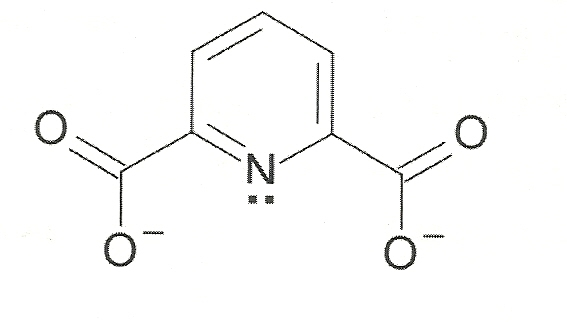
\includegraphics[scale=0.5]{./Figures/dipic.jpg}\\
  \caption{Structure of 2,6-pyridinecarboxylate (dipic)\cite{bib:lab_manual}}\label{fig:dipic}
\end{figure}
 
\subsection{Mechanism}
When $[dipic] >> [CA]$, that is, when $\frac{[dipic]}{[CA]} \ge 25$, then the removal of zinc is pseudo-first-order with respect to CA$\bullet$Zn because the concentration of dipic, denoted as L, does not change appreciably. Thus the formation of the inactive enzyme, apoCA, can be modeled using the following rate equation:
\begin{equation}\label{eqn:a}
\frac{d[\text{apoCA}]}{dt}=k_{obs}[\text{CA$\bullet$Zn}]
\end{equation}
The pseudo-first-order rate constant, $k_{obs}$, increases as [L] increases, but levels off at sufficiently high concentrations of L. Biochemists will recognize behavior similar to Michaelis Menten enzyme kinetics in which the enzyme, CA$\bullet$Zn, and the substrate, L, form a CA$\bullet$Zn$\bullet$L complex with association constant $K_{EML}$ (EML stands for Enzyme-Metal-Ligand). This complex can either revert back to the original species or irreversibly convert to the inactive form of the enzyme, apoCA, and the covalently bound zinc-dipic molecule, ZnL. These two precesses occur as follows:
\begin{align}\label{eqn:KEML_reaction}
\ce{CA$\bullet$Zn + L
<=>[\ce{K_{EML}}]
CA$\bullet$Zn$\bullet$L}
\end{align}
\begin{align}\label{eqn:kd_reaction}
\ce{CA$\bullet$Zn$\bullet$L
->[\ce{k_{d}}]
apoCA + ZnL}
\end{align}